
\documentclass[ ngerman, fontsize= 10pt, headings=big, titlepage=true, xcolor=dvipsnames]{beamer}

\usepackage{babel}
\usepackage[utf8]{inputenc}
\usepackage[T1]{fontenc}
\usepackage{listings}
\lstset{language=R,
    basicstyle=\small\ttfamily,
    stringstyle=\color{OliveGreen},
    otherkeywords={TRUE, FALSE, 0,1,2,3,4,5,6,7,8,9},
    morekeywords={TRUE,FALSE},
    keywordstyle=\color{blue},
    commentstyle=\color{OliveGreen}}
%\usepackage{lmodern, microtype}
\usepackage{csquotes}
\usepackage{hyperref}
\usepackage{enumerate}
\mode<beamer>{
\setbeamertemplate{bibliography item}[book, manual] 
}
%Tablellen:
\usepackage{multirow}
\usepackage{caption}
\usepackage{booktabs}
\usepackage{rotating}
\usepackage{hhline,float}

%Mathematik
\usepackage{amsmath}
\usepackage{amsfonts}
\usepackage{amssymb}
\usepackage{mathtools}
\usepackage{bbm}
\usepackage{color}

%R-Code
\usepackage{xcolor}
\usepackage{wrapfig}


\usetheme{Dresden}
\usecolortheme{spruce}

\title{Grundlagen der Versuchsplanung-Experiment 1}
\subtitle{Längenschätzen}
\author{Kaya Maria Bayer \and Ketevan Gurtskaia \and Alicia Hemmersbach \and Danuscha Große-Hering}
\date{07.Juni 2021}
\begin{document}
\begin{frame}[plain]
    \maketitle
\end{frame}

\begin{frame}{Inhaltsverzeichnis}
	\tableofcontents
\end{frame}

\section{Einleitung}
\begin{frame}{Einleitung}
\begin{itemize}
\item Thema: Längenschätzung
\item bekannt aus TV-Shows z.B. \enquote{Schlag den Star}
\item bei uns: Probanden bekommen zwei verschiedenen Längen gesagt und müssen diese so gut wie möglich nachzeichnen
\end{itemize}
\end{frame}

\section{Problemstellung und Versuchsbedingungen}
\begin{frame}{Ablauf (1/2)}
\underline{Ablauf:}
\begin{itemize}
\item jeder Proband wird einzeln in einen leeren Raum gesetzt
\item in dem Raum steht ein Stuhl und ein leerer, schlichter Tisch 
\item auf diesem liegen ein leerer Zettel und Stift
\item insgesamt gibt es zwei verschiedene Zettelgrößen und zwei verschieden dicke Stiftminen
\item dann werden den Probanden eine Länge mitgeteilt (5cm oder 20cm)
\item die Probanden sollen die Länge auf das Papier zeichnen
\item danach bekommen sie die zweite Länge gesagt
\item einige Probanden bekommen zuerst 5cm gesagt und andere Probanden bekommen zuerst 20cm gesagt



\end{itemize}
	
\end{frame}
\begin{frame}{Ablauf (2/2)}
\begin{itemize}
\item beide Längen werden auf das selbe Papier gezeichnet 
\item drei Personen (Versuchsleiter) aus unserer Gruppe sind für die Mitteilung der Längen zuständig 
\item die vierte Person misst die jeweils gezeichneten Längen der Probanden aus
\end{itemize}
\underline{Problemstellung:}\newline
Können die vorgegebenen Längen genau gezeichnet werden? \newline
Kann eine Länge genauer als die andere Länge gezeichnet werden?

\end{frame}

\section{Analyse des Problems}
\begin{frame}{Analyse des Problems}
	\textbf{1. interessierende abhängige Variable}
	\begin{itemize}
	\item gemessene Längen $x^{i}$ i=5,20
	\end{itemize}
	\textbf{2. interessierende Einflussvariablen}
	\begin{itemize}
	\item genannte Längen $\rightarrow$ zwei Faktorstufen
	\item die Papiergröße (DIN A4, DIN A3)
	\item die Größe der Stiftmine (2mm, 0.5mm)
	\item[$\Rightarrow$] \textbf{Blockvariablen}
	\end{itemize}
\end{frame}
\begin{frame}{Analyse des Problems}
    \textbf{3. mögliche Störvariablen}
    \begin{itemize}
    \item Sehschwächen $\rightarrow$ \textcolor{blue}{nicht vollständig kontrollierbar}
    \item äußere Einflüsse: 
    \begin{itemize}
    \item Lichtverhältnisse $\rightarrow$ \textcolor{blue}{Konstanthaltung}
    \item Ablenkung durch Lärm/andere Personen im Raum \\ $\rightarrow$ \textcolor{blue}{Eliminierung}
    \item Oberfläche des Tisches $\rightarrow$ \textcolor{blue}{Konstanthaltung}
    \end{itemize}
    \item Objekte im Raum, die einem Vergleich dienen könnten $\rightarrow$ \textcolor{blue}{Eliminierung}
   \textcolor{gray}{
    \item Alter, Geschlecht und Rechtshändigkeit der Teilnehmenden
    \item Versuchsleitereffekt
    \item Unterschiede in der Konzentrationsfähigkeit zu verschiedenen Tageszeiten
    }
    \end{itemize}
    
\end{frame}

\section{Modell, Hypothesen und statistische Auswertungsmethoden}
\begin{frame}[fragile]{Modell, Hypothesen und statistische Auswertungsmethoden}
	\begin{itemize}
\item \visible<1->{ $x^{\{ i \}}_1, ....,x^{\{ i \}}_n  $ mit $ i = 5, 20 $ Messungen der gezeichneten Längen}
 \item \visible<1-> {Hypothesen:} 
	\begin{enumerate}
	\item \visible<1-> {$ H_0: \mu^{\{ 5 \}} = 5 $ vs. $H_1: \mu^{\{ 5 \}} \neq 5 $
	\item $H_0: \mu^{\{ 20 \}} = 20 $ vs. $H_1: \mu^{\{ 20 \}} \neq 20 $ }
	\end{enumerate}
\item \visible<2->  {Statistische Tests zum Niveau $\alpha = 0.05 $}
	\end{itemize}
	\begin{enumerate}
  \item[1]<2->  Test auf Normalverteilungsannahme in R mit:  \begin{lstlisting}[language=R]
	shapiro.test(...)
		\end{lstlisting} 
 \item[2a]<2-> Zweiseitiger Einstichproben-t-Test (Normalverteilungsannahme kann nicht abgelehnt werden): \begin{lstlisting}[language=R]
t.test(..., mu = i)$p.value
\end{lstlisting}
 \item[2b]<2-> Zweiseitiger Wilcoxon-Vorzeichen-Rang-Test (Normalverteilungsannahme wird abgelehnt):
 \begin{lstlisting}[language=R]
wilcox.test(..., mu = i)$p.value
\end{lstlisting} 
	\end{enumerate}

\end{frame}

\begin{frame}[fragile]
\begin{Definition}[Transformation der Messwerte]
Transformation der Messwerte bedeutet, dass statt der Messwerte selbst eine Größe verwendet wird, die sich durch eine einfache Umrechnung aus den Messwerten ergibt. Für alle weiteren Analysen werden dann diese umgerechneten Werte verwendet. (Kleppmann  2020, S.95)
\end{Definition}
\begin{itemize}
\item Transformierte Werte:$y^{\{ i \}}_1, ....,y^{\{ i \}}_n  $, $ i = 5, 20 $
\item $y^{\{i \}}_j := \frac{x^{\{i\}}_j - i}{i} $ mit $j = 1, ..., n.$ \quad $ i = 5, 20 $
\item  $ \tilde{\mu} ^{\{5\}} := \frac{\mu ^{\{5\}} - 5}{5} $, \quad $\tilde{\mu} ^{\{20\}} := \frac{\mu ^{\{20\}} - 20}{20} $
\item Testfrage: Kann eine der vorgegebenen Längen besser hergestellt werden? 

\end{itemize}


\end{frame}
\begin{frame}[fragile]
\begin{itemize}
\item <1-> Hypothesen:
 $ H_0: \tilde{\mu}^{\{ 5 \}} -\tilde{\mu}^{\{ 20 \}}  = 0  $ vs. $H_1: \tilde{\mu}^{\{ 5 \}} -\tilde{\mu}^{\{ 20 \}}  \neq 0 $
bzw.  $H_0: \tilde{\mu}^{\{ 5 \}} =\tilde{\mu}^{\{ 20 \}}  $ vs. $H_1: \tilde{\mu}^{\{ 5 \}} \neq \tilde{\mu}^{\{ 20 \}} $
\item[1]<1->  Test auf Normalverteilungsannahme in R mit:  \begin{lstlisting}[language=R]
shapiro.test(y5 - y20)
\end{lstlisting} 
\item[2a]<2-> Normalverteilung nicht abgelehnt $\rightarrow $ auf Varianzhomogenität testen: $H_0: \sigma_1 = \sigma_2 $ vs. $ H_1: \sigma_1 \neq \sigma_2 $ mit:
\begin{lstlisting}[language=R]
var.test(y5, y20, alternative="two.sided")
\end{lstlisting} 
Zweiseitige Zweistichproben-t-Tests:
\item[2a.1]<2-> Annahme der Varianzhomogenität bleibt beibehalten: 
\begin{lstlisting}[language=R]
t.test(y5, y20, paired = TRUE, var.equal = TRUE )
\end{lstlisting} 
\item[2a.2]<2-> Signifikante Abweichung von der Annahme: 
\begin{lstlisting}[language=R]
t.test(y5, y20, paired = TRUE, var.equal = FALSE)
\end{lstlisting} 
\item[2b]<2-> Keine Normalverteilung: Zweistichproben-Wilcoxon-Test
\begin{lstlisting}[language=R]
wilcox.test(y5 - y20)$p.value
\end{lstlisting} 
\end{itemize}
\end{frame}

\section{Versuchsplanung}
\begin{frame}{Beschreibung der Versuchsplanung}
\begin{itemize}
\item Maximierung der Variation  der Einflussvariable : Jede Stufe kommt gleich häufig vor.\\
\item Minimierung der Störvariablen: Möglichst gleiche sonstigen Versuchsbedingungen: alle Teilnehmenden im gleichen Raum (aber alleine), gleiche Anweisungen	(Konstanthaltung der Störvariablen)
\item Identifizierbarkeit: alle Stufenkombinationen werden durchgeführt
\end{itemize}
\end{frame}

\begin{frame}[fragile]{Versuchsplan}
	\textbf{1. Grafische Bestimmung der minimalen Stichprobengröße}\\
	$\alpha =0.05$, $\beta = 0.95$ und $\delta =1$\\
	 Betrachte die Stichprobengröße n $\in [1,28]$
	 

	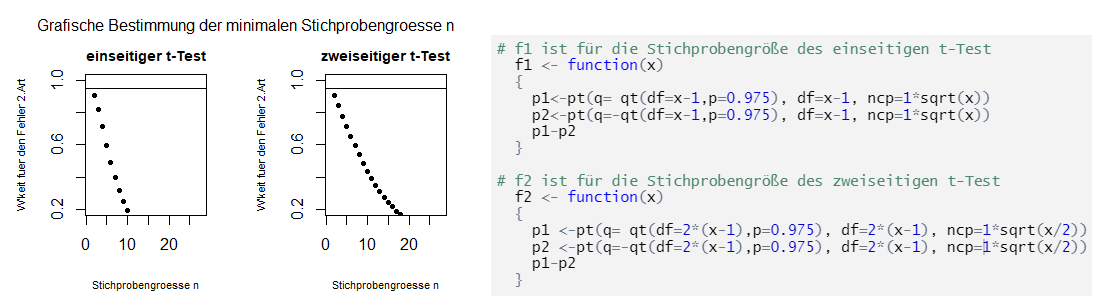
\includegraphics[scale=0.4]{Stichprobengröße.png}
 


	$\Rightarrow n > 0$
\end{frame}

\begin{frame}{Versuchsplan (2/4)}
	
	
	\begin{itemize}
		\item Faktor: Reihenfolge der Länge (2 Stufen)
		\item Block: Papiergröße (2 Stufen), Stiftgröße(2 Stufen)	
		\item balanzierten Versuchsplan\\
		 $\Rightarrow n = S_{Faktor} \cdot S_{Block\ A} \cdot  S_{Block\ B} \cdot k =2 \cdot 2\cdot 2\cdot k = 8\cdot k$ \\
		 mit k $\in \mathbb{N}_+$
		
		\item mögliche Probanden =28 $\Rightarrow$ k = 3 $\Rightarrow$ n=24 (Zufällig)
		\item Fehler 2.Art mit n=24 : ca.0.35 (einseitiger t-Test), ca.0.6 (zweiseitiger t-Test)
		
		
	\end{itemize}
	
\end{frame}
\begin{frame}[fragile]{Versuchsplan (3/4)}
	
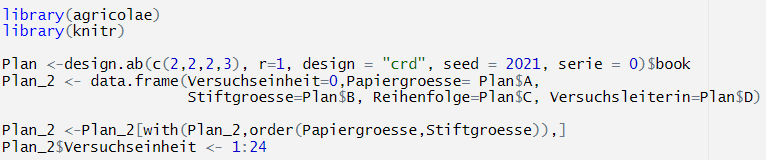
\includegraphics[scale=0.7]{Code_Versuchsplan.png}

{\small
\begin{table}[hb]
	\caption{Versuchsplan 1.Hälfte}
	\centering
	\begin{tabular}[b]{l||l|l|l|l|l|l|l|l|l|l|l|l}
		\hline
		Einheit & 1 & 2 & 3 & 4 & 5 & 6 & 7 & 8 & 9 & 10 & 11 & 12\\
		\hhline{=============}
		Block A & 1 & 1 & 1 & 1 & 1 & 1 & 1 & 1 & 1 & 1 & 1 & 1\\
		\hline
		Block B & 1 & 1 & 1 & 1 & 1 & 1 & 2 & 2 & 2 & 2 & 2 & 2\\
		\hline
		Faktor & 2 & 2 & 2 & 1 & 1 & 1 & 2 & 2 & 1 & 1 & 1 & 2\\
		\hhline{=============}
		{\tiny Versuchsleiterin} & 1 & 3 & 2 & 3 & 1 & 2 & 2 & 3 & 2 & 1 & 3 & 1\\
		\hline
	\end{tabular}
\end{table}}

\end{frame}
\begin{frame}{Versuchsplan (4/4)}
	
{\small
\begin{table}[hb]
	\caption{Versuchsplan 2.Hälfte}
	\centering
	\begin{tabular}[b]{l||l|l|l|l|l|l|l|l|l|l|l|l}
		\hline
		Einheit & 13 & 14 & 15 & 16 & 17 & 18 & 19 & 20 & 21 & 22 & 23 & 24\\
		\hhline{=============}
		Block A & 2 & 2 & 2 & 2 & 2 & 2 & 2 & 2 & 2 & 2 & 2 & 2\\
		\hline
		Block B & 1 & 1 & 1 & 1 & 1 & 1 & 2 & 2 & 2 & 2 & 2 & 2\\
		\hline
		Faktor & 2 & 1 & 1 & 2 & 2 & 1 & 2 & 1 & 1 & 1 & 2 & 2\\
		\hhline{=============}
		{\tiny Versuchsleiterin} & 3 & 2 & 3 & 1 & 2 & 1 & 2 & 2 & 3 & 1 & 1 & 3\\
		\hline
	\end{tabular}
\end{table}}

\begin{itemize}
	\item Block A $\hat{=}$ Papiergröße mit zwei Stufen: 1:= A4 und 2:= A3  
	\item Block B $\hat{=}$ Stiftgröße auch mit zwei Stufen:  1:= 0.5mm und 2:=2mm 
	\item Faktor $\hat{=}$ Reihenfolge der Längen: 1:= zuerst 5cm und 2:= zuerst 20cm
\end{itemize}

\end{frame}



\section{Literaturverzeichnis}
\begin{frame}{Literaturverzeichnis}
\begin{thebibliography}{Kleppmann}
\setbeamertemplate{bibliography item}[book]
 \bibitem{Kleppmann}
 Kleppmann, Wilhelm, (2020),
 \newblock Versuchsplanung, 10. Aufl., 
\newblock Carl Hanser Verlag,
München.
\setbeamertemplate{bibliography item}[manual]
\bibitem{R}
Die statistischen
Berechnungen wurden mit R 3.6.3 durchgeführt
\newblock (R Development Core Team 2020) 
 \end{thebibliography}
\end{frame}

\end{document}
